%\documentclass[draft,grl]{AGUTeX}
\documentclass[twocolumn,grl]{AGUTeX}
\usepackage{mathptmx}
% \usepackage{lineno}
% \linenumbers*[1]

%  To add line numbers to lines with equations:
%  \begin{linenomath*}
%  \begin{equation}
%  \end{equation}
%  \end{linenomath*}

%  Uncomment the following command to include .eps files
%  (comment out this line for draft format):
%\usepackage[dvips]{graphicx}
\usepackage[pdftex]{graphicx}
%\setkeys{Gin}{draft=false}

\authorrunninghead{STYRON AND HETLAND}
\titlerunninghead{LANF EARTHQUAKE LIKELIHOOD}

\authoraddr{Corresponding author: Richard H. Styron,
Department of Earth and Environmental Sciences, University of
Michigan, 2534 CC Little Bldg., 1100 N. University Ave., 
Ann Arbor, MI 48104, USA (richard.h.styron@gmail.com)}

\begin{document}
\title{Likelihood of observing an earthquake on a low-angle normal fault}

\authors{Richard H. Styron \altaffilmark{1}
and Eric A. Hetland \altaffilmark{1}}

\altaffiltext{1}{Department of Earth and Environmental Sciences, University of
Michigan, Ann Arbor, Michigan, USA.}

\begin{abstract}
rothko
\end{abstract}

\begin{article}

\section{Introduction}
The recognition of low-angle normal faults, or LANFs, with fault dips less than 30$^\circ$ in the geologic record and their hypothesized role in accommodating large-magnitude continental extension [1] has been one of the most important developments in tectonics over the past several decades.
However, despite widespread field observations of inactive LANFs[2] and their central role in modern extensional tectonic theory[3], they remain enigmatic and contentious structures. 
This is for two reasons: because brittle faulting on LANFs is in apparent conflict with standard rock mechanical theory as typically applied to the upper crust [4,5], and because observations of active faulting on LANFs is sparse and at times ambiguous[6,7].
A considerable amount of research has been performed to address the former concern, reconciling LANF slip with rock mechanics.
The latter issue, the paucity of observations, has inhibited hypothesis testing of LANF fault theory, and has also contributed to a mode of thought where the absence of evidence for LANF activity is taken as evidence of its absence [8, 9].
Alternately, the lack of observed seismic slip on a continental LANF may be explained by the rarity of seismicity and the small number of potential active structures.


In this work, we choose to directly address the question of whether the lack of observed seismicity may be interpreted as an indication that LANFs may not slip seismically, or is an effect of a small sample size of LANFs that show typical seismic behavior.  We do this by calculating the likelihood of observing a moderate to large earthquake on a LANF over different time windows, assuming that all continental LANFs described in the literature are seismically active at low angles and display typical seismic behavior.

\section{Potentially Active LANFs}

Over the past decade or so, many field studies have found evidence for LANF activity in orogens throughout the world. These studies typically find arrays of Quaternary normal fault scarps on the fault traces and/or in the hanging walls of mapped or inferred low-angle detachment faults [e.g, Axen et al., 1999]. Some studies also have bedrock thermochronology data from the exhumed footwalls of the detachments that is suggestive of ongoing rapid exhumation [e.g. Sundell et al., 2013], although this data does not preclude a recent cessation of faulting. In some cases, additional evidence for LANF activity comes from geophysical data such as GPS geodesy [Hreinsdottir and Bennett, 2009] and seismic waves [Doser, 1987].

We have compiled all potentially active LANFs with known subareal fault traces from a thorough review of the literature; there are nineteen total (Figure~\ref{fig:lanf_map}).  About half are in Tibet, consistent with hypotheses that LANF and metamorphic core complexes form in areas of hot, thick crust [e.g., Buck, 1988].  The rest are distributed through other areas of active continental extension: the North American Basin and Range, the Malay Archipelago, Turkey, Italy, and Peru. Several of the most-commonly cited candidates for seismically active LANFs were not included because they do not have a clearly-defined, mappable fault trace, which is necessary for our calculations.  These include the submarine core complexes in the Woodlark Basin [Abers, 2001], the fault responsible for the 1995 Aigion, Greece earthquake [Bernard et al., 1997] and other potential LANFs underneath the Gulf of Corinth, and the fault responsible for the 1952 Ancash, Peru earthquake [Doser, 19xx].

We have then mapped the approximate fault traces into a GIS file (available at https://github.com/cossatot/LANF\_gis), with metadata such as slip rate and source. We then have estimated the probability of observing an earthquake above a given magnitude for each fault individually over some time window, and then calculated the probability of observing a significant earthquake on any of the faults over that same time window.

\section{Likelihood of observing a LANF earthquake}
\subsection{Rupture Likelihood on Individual LANFs}
To estimate the likelihood of observing a significant earthquake on an individual LANF over some contiguous time window of length $t$ (in years), we perform a Monte Carlo simulation in which we create 2000 synthetic time series of earthquakes, with unique values for fault geometry and slip rate for each time series. Then, for each time series we calculate the fraction of unique time windows of length $t$ in which an earthquake as large or larger than a given magnitude occurs.  We take this value as the probability of observing an earthquake.  This value is then multiplied by the fraction of the total range of fault dip which is at or below 30$^\circ$, as many of the faults studied have possible dips above 30$^\circ$.

Each earthquake sequence is generated by randomly sampling 50,000 events from a tapered Gutenberg-Richter distribution with corner magnitude $M_c = 7.64$ and $\beta = 0.65$ (from values estimated by Bird and Kagan [2004] for continental rifts) using an inverse transform sampling algorithm.  The samples are taken from a moment magnitude interval $M = [5.0, \, M_{max}]$, where $M_{max}$ is calculated as the magnitude M resulting from fault slip $D$ = 15 m over a fault of length $L$ cutting through a seismogenic thickness $z$ at dip $\delta$, given the relations $ M_o = \mu L z D \,/ \, \sin \delta $ and $ M = 2/3 \; \log_{10} (M_o) - C $, where $C = 6 $ and shear modulus $\mu = 30$ GPa.  Sensitivity tests (see Supplementary Materials) show that the results are only slightly affected by the frequency-magnitude distribution: differences between results using this distribution and a `characteristic' distribution with an enhanced probability of earthquakes around $M$ 6 are well below the variability created by uncertainty in fault dip and slip rate.

Then, a time series of strain accumulation and release for each earthquake sequence is created, with one value per year.  This is constructed by separating each earthquake from the previous one with a set of zeros (representing no significant earthquakes for those years) where the number of zero years before an event corresponds to the length of an interseismic interval necessary to accumulate all the slip released in that event, given the fault dimensions and slip rate for that time series. Then, the likelihood of observing a significant earthquake is calculated as described above.

\subsection{Probability on All LANFs}
To calculate the probability of observing an earthquake over the time window on any of the LANFs studied, we first assume that seismicity on each fault is independent and uncorrelated from seismicity on all other faults. This assumption is likely true for most faults, but may not be true for some proximal faults (such as the North and South Lunggar detachments, or the Papangeo and Tokorondo detachments), though it is hard to determine how these faults may interact.  Then, we determine the probability  
\begin{equation}
p_{AT \, or \, LP\, \ldots \, or \, DV} = 1 - (q_{AT} \cdot q_{LP} \cdot \ldots \, \cdot q_{DV})
\end{equation}
where $p_{AT}$ is the probability of observing an earthquake on a single LANF (the Alto-Tiberina fault), and $q_{AT} = 1 - p_{AT}$.

\appendix
\section{Do I need an appendix?}
The function of your appendix is ambiguous at best and probably unnecessary.

\begin{acknowledgments}
We thank Jon Spencer for a stimulating discussion that lead to this work.

\end{acknowledgments}

\end{article}

\begin{figure}
\noindent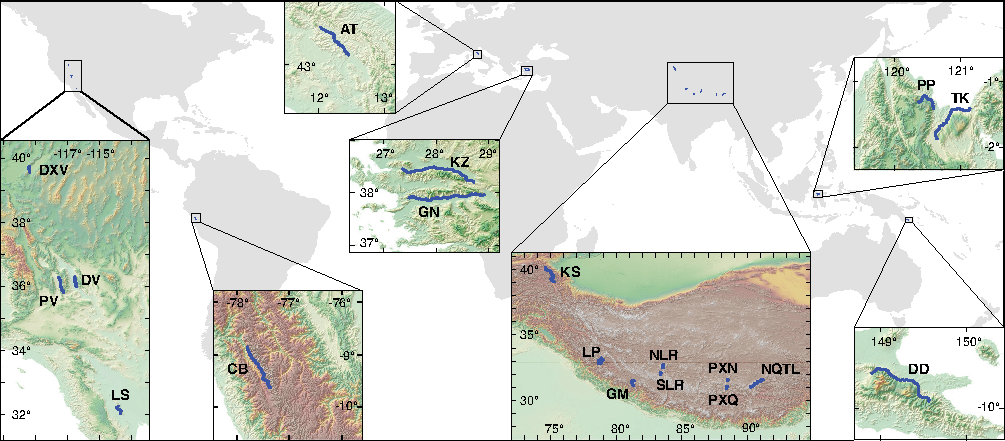
\includegraphics[width=40pc]{figures/active_lanfs_map_insets.pdf}
\caption{Map of known, potentially active continental LANFs (blue lines), with insets showing the physiographic context of the faults.  DXV=Dixie Valley fault.  PV=Panamint Valley fault.  DV=Death Valley fault.  LS=Laguna Salada fault.  CB=Cordillera Blanca detachment.  AT=Alto-Tiberina fault.  KZ=Kuzey detachment.  GN=Guney detachment.  KS=Kongur Shan fault.  LP=Leo Pargil detachment.  GM=Gurla Mandhata detachment. NLR=North Lunggar detachment.  SLR=South Lunggar detachment.  PXN=Pum Qu--Xainza north fault.  PXQ=Pum Qu--Xainza Qingdu fault.  NQTL=Nyainqentanglha detachment.  PP=Papangeo detachment.  TK=Tokorondo detachment.  DD=Dayman Dome.}
\label{fig:lanf_map}
\end{figure}


\end{document}


